% LEFT SIDE ====================================================
\draw[color=gray!50, fill=gray!50] (1, 1) rectangle (7, 28.7);
\draw[color=white, fill=white] (4, 26) circle (2.2cm);
% Graphic: Photo
\node[circle,draw,
           text=white,
           fill=white,
           text width=4cm,
           path picture={
               \node at (path picture bounding box.center){
                   
\includegraphics[width=4cm]{pictures/noimage} % INPUT
               };
           }] at (4, 26) {};


\foreach \y in {22}{
  % Contact =============
  \node[anchor=west, colorDark, thick] at (1.5, \y ) {\Large \textsc{Contact}}; % INPUT
  \draw[colorDark, very thick] (4 ,22) -- (6.5 , \y );

  % Date of Birth
  \node[circle,draw,
              text width=.5cm,
              fill=white,
              inner sep=0pt,
              path picture={
                  \node at (path picture bounding box.center){
                      
\includegraphics[width=.5cm]{pictures/contact} % INPUT
                  };
              }] at (1.75, \y - 1) {};

  \node[anchor=west, colorDark, thick] at (2.25, \y - 1) {\large 06.11.1986, Bielefeld}; % INPUT

  % Location
  \node[circle,draw,
              text width=.5cm,
              fill=white,
              inner sep=0pt,
              path picture={
                  \node at (path picture bounding box.center){
                      
\includegraphics[width=.5cm]{pictures/location} % INPUT
                  };
              }] at (1.75, \y - 2) {};

  \node[anchor=west, colorDark, thick] at (2.25, \y - 2) {\large Frankurt am Main}; % INPUT

  % Phone
  \node[circle,draw,
              text width=.5cm,
              fill=white,
              inner sep=0pt,
              path picture={
                  \node at (path picture bounding box.center){
                      
\includegraphics[width=.5cm]{pictures/phone2} % INPUT
                  };
              }] at (1.75, \y - 3) {};

  \node[anchor=west, colorDark, thick] at (2.25, \y - 3) {\large +49 69 / 0170 180 7175}; % INPUT

  % E-Mail
  \node[circle,draw,
              text width=.5cm,
              fill=white,
              inner sep=0pt,
              path picture={
                  \node at (path picture bounding box.center){
                      
\includegraphics[width=.5cm]{pictures/mail} % INPUT
                  };
              }] at (1.75, \y - 4) {};

  \node[anchor=west, colorDark, thick] at (2.25, \y - 4) {\large \href{mailto:jfk.lorenz@gmail.com}{jfk.lorenz@gmail.com}}; % INPUT

  % GitHub
  \node[circle,draw,
              text width=.5cm,
              fill=white,
              inner sep=0pt,
              path picture={
                  \node at (path picture bounding box.center){
                      
\includegraphics[width=.5cm]{pictures/git} % INPUT
                  };
              }] at (1.75, \y - 5) {};

  \node[anchor=west, colorDark, thick] at (2.25, \y - 5) {\large \href{https://github.com/jfklorenz/}{GitHub: jfklorenz}}; % INPUT
}

\foreach \y in {15.5}{
  % Languages =============
  \node[anchor=west, colorDark, thick] at (1.5, \y) {\Large \textsc{Languages}}; % INPUT
  \draw[colorDark, very thick] (4.5, 15.5) -- (6.5, \y);

  % German
  \node[circle,draw,
              text width=.5cm,
              fill=white,
              inner sep=0pt,
              path picture={
                  \node at (path picture bounding box.center){
                      
\includegraphics[width=.5cm]{pictures/ger} % INPUT
                  };
              }] at (1.75, \y - 1) {};
  \node[anchor=west, colorDark, thick] at (2.25, \y - 1) {\large Native speaker}; % INPUT


  % English
  \node[circle,draw,
              text width=.5cm,
              fill=white,
              inner sep=0pt,
              path picture={
                  \node at (path picture bounding box.center){
                      
\includegraphics[width=.5cm]{pictures/eng} % INPUT
                  };
              }] at (1.75, \y - 2) {};

  \node[anchor=west, colorDark, thick] at (2.25, \y - 1.75) {\large Fluent}; % INPUT
  \node[anchor=west, colorDark, thick] at (2.25, \y - 2.25) {(Camebridge Certificate)}; % INPUT


  % French
  \node[circle,draw,
              text width=.5cm,
              fill=white,
              inner sep=0pt,
              path picture={
                  \node at (path picture bounding box.center){
                      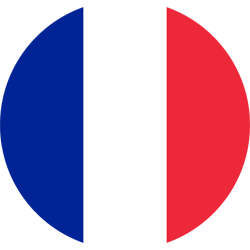
\includegraphics[width=.5cm]{pictures/fra} % INPUT
                  };
              }] at (1.75, \y - 3) {};
  \node[anchor=west, colorDark, thick] at (2.25, \y - 3) {\large Basic knowledge}; % INPUT
}

\foreach \y in {11}{
  % Skills =============
  \node[anchor=west, colorDark, thick] at (1.5, \y) {\Large \textsc{Skills}}; % INPUT
  \draw[colorDark, very thick] (3.35, \y) -- (6.5, \y);

  % Python
  \node[colorDark, anchor=west] at (1.5, \y - 1) {Python}; % INPUT
  \node[colorDark, anchor=east] at (6.5, \y - 1) {\footnotesize $90\%$}; % INPUT
  \draw[color=black, fill=white] (1.5, \y - 1.5) rectangle (6.5, \y - 1.25); % INPUT
  \draw[fill=black!80] (1.5, \y - 1.5) rectangle (6, \y - 1.25); % INPUT

  % Javascript
  \node[colorDark, anchor=west] at (1.5, \y - 2) {Javascript}; % INPUT
  \node[colorDark, anchor=east] at (6.5, \y - 2) {\footnotesize $75\%$}; % INPUT
  \draw[color=black, fill=white] (1.5, \y - 2.5) rectangle (6.5, \y - 2.25); % INPUT
  \draw[fill=black!80] (1.5, \y - 2.5) rectangle (5.25, \y - 2.25);

  % LaTeX
  \node[colorDark, anchor=west] at (1.5, \y - 3) {SQL}; % INPUT
  \node[colorDark, anchor=east] at (6.5, \y - 3) {\footnotesize $80\%$}; % INPUT
  \draw[color=black, fill=white] (1.5, \y - 3.5) rectangle (6.5, \y - 3.25); % INPUT
  \draw[fill=black!80] (1.5, \y - 3.5) rectangle (5.5, \y - 3.25); % INPUT

  % SQL
  \node[colorDark, anchor=west] at (1.5, \y - 4) {Git}; % INPUT
  \node[colorDark, anchor=east] at (6.5, \y - 4) {\footnotesize $80\%$}; % INPUT
  \draw[color=black, fill=white] (1.5, \y - 4.5) rectangle (6.5, \y - 4.25); % INPUT
  \draw[fill=black!80] (1.5, \y - 4.5) rectangle (5.5, \y - 4.25); % INPUT

  % Matlab
  \node[colorDark, anchor=west] at (1.5, \y - 5) {Matlab}; % INPUT
  \node[colorDark, anchor=east] at (6.5, \y - 5) {\footnotesize $75\%$}; % INPUT
  \draw[color=black, fill=white] (1.5, \y - 5.5) rectangle (6.5, \y - 5.25); % INPUT
  \draw[fill=black!80] (1.5, \y - 5.5) rectangle (5.25, \y - 5.25); % INPUT

  % R
  \node[colorDark, anchor=west] at (1.5, \y - 6) {R}; % INPUT
  \node[colorDark, anchor=east] at (6.5, \y - 6) {\footnotesize $70\%$}; % INPUT
  \draw[color=black, fill=white] (1.5, \y - 6.5) rectangle (6.5, \y - 6.25); % INPUT
  \draw[fill=black!80] (1.5, \y - 6.5) rectangle (5, \y - 6.25); % INPUT

  % LaTeX
  \node[colorDark, anchor=west] at (1.5, \y - 7) {\LaTeX}; % INPUT
  \node[colorDark, anchor=east] at (6.5, \y - 7) {\footnotesize $95\%$}; % INPUT
  \draw[color=black, fill=white] (1.5, \y - 7.5) rectangle (6.5, \y - 7.25); % INPUT
  \draw[fill=black!80] (1.5, \y - 7.5) rectangle (6.25, \y - 7.25); % INPUT
}
